\documentclass[a4paper,12pt]{report}
\usepackage[utf8]{inputenc}
\usepackage[francais]{babel}
\usepackage{fancyhdr}
\usepackage{graphicx}
\usepackage{tikz}
\usetikzlibrary{calc}
\usepackage{listings}
\usepackage{xcolor}
\definecolor{grey}{rgb}{0.9,0.9,0.9}
\usepackage{titlesec}
\usepackage{verbatim}
\usepackage{listings}
\usepackage{textcomp}
\usepackage{hyperref}
\usepackage{longtable}
\usepackage{colortbl}
\usepackage{amssymb}

\definecolor{javakeyword}{rgb}{0,0,0.5}
\definecolor{javastring}{rgb}{0,0.5,0}
\definecolor{javacomment}{rgb}{0.5,0.5,0.5}
\lstdefinestyle{C++}{
   language=C++, basicstyle=\footnotesize,       % the size of the fonts that are used for the code
  numbers=left,                   % where to put the line-numbers
  numberstyle=\tiny\color{gray},  % the style that is used for the line-numbers
  stepnumber=1,                   % the step between two line-numbers. If it's 1, each line
                                  % will be numbered
  numbersep=5pt,                  % how far the line-numbers are from the code
  backgroundcolor=\color{white},  % choose the background color. You must add \usepackage{color}
  showspaces=false,               % show spaces adding particular underscores
  showstringspaces=false,         % underline spaces within strings
  showtabs=false,                 % show tabs within strings adding particular underscores
  frame=single,                   % adds a frame around the code
  rulecolor=\color{black},        % if not set, the frame-color may be changed on line-breaks within not-black text (e.g. commens (green here))
  tabsize=2,                      % sets default tabsize to 2 spaces
  captionpos=b,                   % sets the caption-position to bottom
  breaklines=true,                % sets automatic line breaking
  breakatwhitespace=false,        % sets if automatic breaks should only happen at whitespace
  title=\lstname,                 % show the filename of files included with \lstinputlisting;
   stringstyle=\color{javastring},
   keywordstyle=\color{javakeyword}\ttfamily\textbf,
   commentstyle=\color{javacomment}\ttfamily\textit
 }
\frenchbsetup{StandardLists=true}
\newcommand{\marge}{18mm}
\usepackage[left=\marge,right=\marge,top=\marge,bottom=\marge]{geometry}
\pagestyle{fancy}
\setlength{\headheight}{15pt}
\renewcommand{\headrulewidth}{1pt}
\linespread{1}
\setlength{\columnseprule}{0.2pt}
\title{TP2 VISA : reconstruction 3D, géométrie épipolaire et stéréovision}
\author{NAIT ABDELAZIZ Yanis}


\begin{document}
\maketitle
\section*{Introduction}
Dans ce TP, nous allons utiliser le principe de stéréovision afin d'identifier les paires de points similaires deux images  d'un objet prises par une même caméra sous deux angles différents. On peut voir ci-dessous les deux images sur lesquels nous allons procéder à l'identification de ces paires de points:
\begin{figure}[!ht]
	\center
	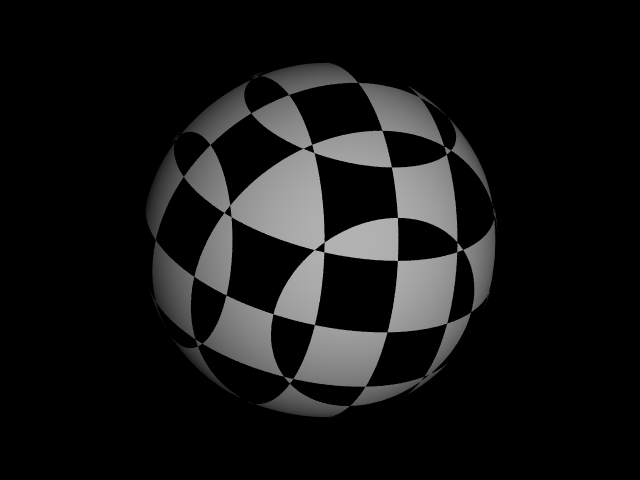
\includegraphics[scale=0.3]{image/left.png}
	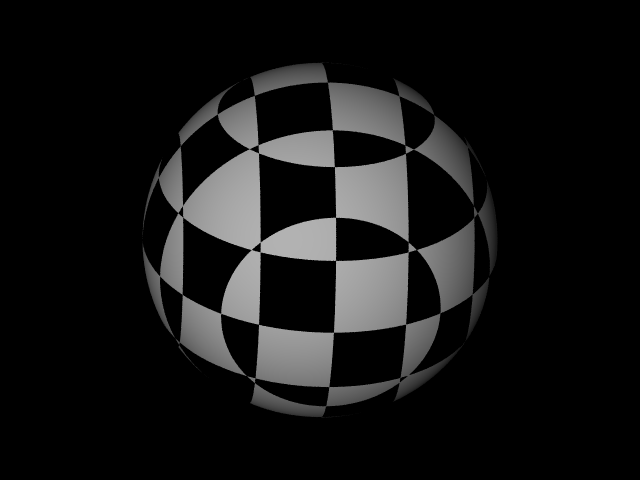
\includegraphics[scale=0.3]{image/right.png}
\end{figure}

\section*{I-Calcul de la matrice fondamentale}
Dans cette partie de TP, nous allons déterminer la matrice fondamentale permettant de calculer l'image d'un point dans le repère de l'image de gauche dans le repère de l'image de droite. L'image d'un point dans  l'image gauche est appelée droite épipolaire dans l'image droite correspondante à ce point.
\subsubsection*{1-Produit vectoriel}

\noindent Avant de pouvoir calculer la matrice fondamentale , nous devons d'abord écrire le code de la fonction permettant de décrire le produit vectoriel d'un vecteur. Ainsi une combinaison linéaire des matrices intrinsèques et extrinsèques des deux caméras avec un produit vectoriel pourra être considérée comme une homographie.
La fonction ci-dessous permet de calculer rapidement le produit vectoriel d'un vecteur par lui-même 
\begin{lstlisting}[style=C++]
Mat iviVectorProductMatrix(const Mat& v) {

    Mat mVectorProduct = Mat::eye(3, 3, CV_64F);

    mVectorProduct.at<double>(0,0) = (double)0.0;
    mVectorProduct.at<double>(0,1) = -v.at<double>(2,0);
    mVectorProduct.at<double>(0,2) = v.at<double>(1,0);

    mVectorProduct.at<double>(1,0) = v.at<double>(2,0);
    mVectorProduct.at<double>(1,1) = (double)0.0;
    mVectorProduct.at<double>(1,2) = -v.at<double>(0,0);

    mVectorProduct.at<double>(2,0) = -v.at<double>(1,0);
    mVectorProduct.at<double>(2,1) = v.at<double>(0,0);
    mVectorProduct.at<double>(2,2) = (double)0.0;

    return mVectorProduct;
}
\end{lstlisting}
\subsubsection*{2-Matrice fondamentale}
\noindent Le code ci-dessous permet de calculer la matrice fondamentale permettant de calculer l'image d'un point d'un repère dans un autre repère. L'image d'un point ainsi obtenue est la droite épipolaire associée à ce point dans l'autre repère.
\begin{lstlisting}[style=C++]
Mat iviFundamentalMatrix(const Mat& mLeftIntrinsic,
                         const Mat& mLeftExtrinsic,
                         const Mat& mRightIntrinsic,
                         const Mat& mRightExtrinsic) {
    
    Mat mFundamental = Mat::eye(3, 3, CV_64F);

    Mat pLeft = mLeftIntrinsic * Mat::eye(3, 4, CV_64F) * mLeftExtrinsic;
    Mat pRight = mRightIntrinsic * Mat::eye(3, 4, CV_64F) * mRightExtrinsic;

    Mat o1 = mLeftExtrinsic.inv().col(3);
    Mat a = pRight*o1;
    Mat b = pRight*pLeft.inv(DECOMP_SVD);

    mFundamental = iviVectorProductMatrix(a)*b;

    return mFundamental;
}
\end{lstlisting}
\noindent Pour obtenir l'image d'un point d'un repère R1 dans le plan R2, on multiplie ses coordonnées par cette matrice fondamentale et l'image d'un point dans le plan R2, on multiplie ses coordonnées par la transposée inverse de cette matrice fondamentale.

\section*{II-Extraction des coins}
\noindent Dans cette partie, nous allons extraire des deux images des pixels d'intérêt qu'on appelle coins et qui serviront pour la mise en correspondance de ces deux images. Le code ci-dessous permet grâce à une fonction développée dans la bibliothèque opencv d'extraire ces points qu'on stockera dans deux matrices correspondantes aux deux images.
\begin{lstlisting}[style=C++]
Mat iviDetectCorners(const Mat& mImage,
                     int iMaxCorners){
    vector<Point2f> vCorners;

    goodFeaturesToTrack(mImage,vCorners,iMaxCorners,0.01,10,Mat(),3,false,0.04);
    Mat mCorners(3,vCorners.size(),CV_64F);
    for(int i=0;i<vCorners.size();i++){
        mCorners.at<double>(0,i)=(double)vCorners[i].x;
        mCorners.at<double>(1,i)=(double)vCorners[i].y;
        mCorners.at<double>(2,i)=1;
    }
    return mCorners;
}
\end{lstlisting}
\noindent Après extraction de ces points d'intérêts , on obtient les points mis en évidence en rouge sur les deux images suivantes ainsi que les lignes en vert qui représentent les droites épipolaires associées à ces points.
\begin{figure}[!ht]
	\center
	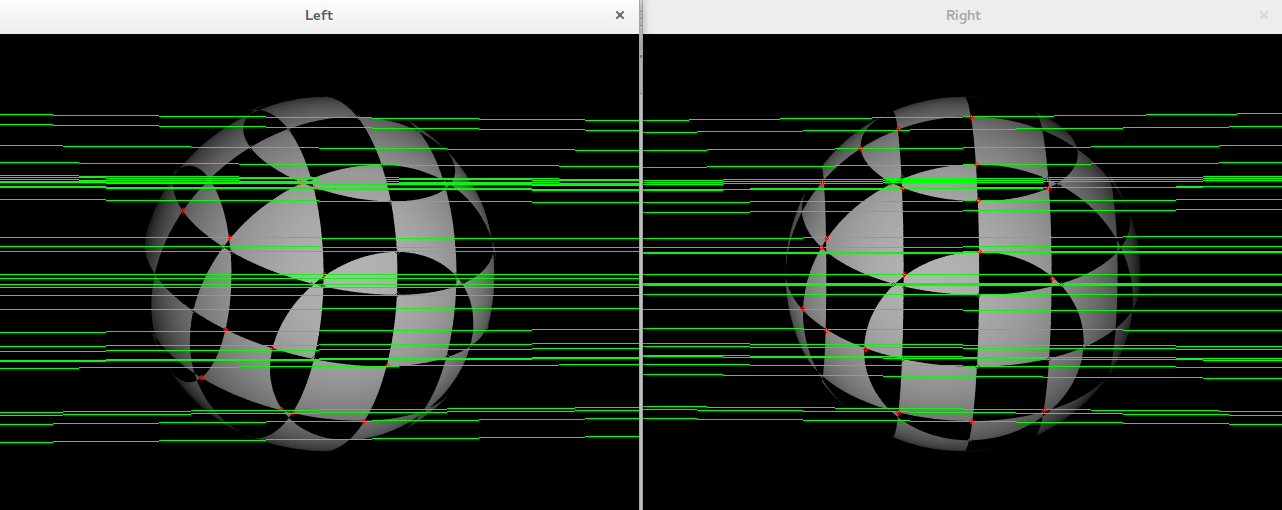
\includegraphics[scale=0.3]{image/coins.png}
\end{figure}
\section*{III-Calcul des distances}
Pour déterminer la meilleure correspondance entre les points des deux images , pour chaque point d'une image nous allons calculer sa distance par rapport à toutes droites épipolaires associées aux points de l'autre image que l'on stockera dans une matrice bi-dimensionnelle comme ci-suivant :\\
\[
	distances=\left (
	\begin{array}{ccc}
		d(l1,epi(r1))+d(epi(l1),r1) & ...    & d(l1,epi(rm))+d(epi(l1),rm)    \\
		...    & ... & ...   \\
		d(ln,epi(r1))+d(epi(ln),r1)    & ... & d(ln,epi(rm))+d(epi(ln),rm)    \\
	\end{array}
	\right )
\]
\noindent Le code ci-dessous permet ainsi de calculer cette matrice de distances.

\begin{lstlisting}[style=C++]
Mat iviDistancesMatrix(const Mat& m2DLeftCorners,
                       const Mat& m2DRightCorners,
                       const Mat& mFundamental){
    double x1,y1,z1,x2,y2,z2,d1,d2;
    Mat epiDroite,epiGauche,point1,point2;
    int widthL,widthR;

    widthL = m2DLeftCorners.size().width;
    widthR = m2DRightCorners.size().width;

    Mat mDistances(widthL,widthR,CV_64F);

    for(int i=0;i<widthL;i++){

          x1 = m2DLeftCorners.at<double>(0,i);
          y1 = m2DLeftCorners.at<double>(1,i);
          z1 = m2DLeftCorners.at<double>(2,i);

          point1 = (Mat_<double>(3,1) << x1,y1,z1);

          epiDroite = mFundamental*point1;

          for(int j=0;j<widthR;j++){

               x2 = m2DRightCorners.at<double>(0,j);
               y2 = m2DRightCorners.at<double>(1,j);
               z2 = m2DRightCorners.at<double>(2,j);

               point2 = (Mat_<double>(3,1) << x2,y2,z2);
               epiGauche = mFundamental.t()*point2;

               d1 = abs(epiDroite.at<double>(0,0)*x2+epiDroite.at<double>(1,0)*y2+epiDroite.at<double>(2,0))/
                    (sqrt(epiDroite.at<double>(0,0)*epiDroite.at<double>(0,0)+epiDroite.at<double>(1,0)*epiDroite.at<double>(1,0)));

               d2 = abs(epiGauche.at<double>(0,0)*x1+epiGauche.at<double>(1,0)*y1+epiGauche.at<double>(2,0))/
                    (sqrt(epiGauche.at<double>(0,0)*epiGauche.at<double>(0,0)+epiGauche.at<double>(1,0)*epiGauche.at<double>(1,0)));

               mDistances.at<double>(i,j)=d1+d2;
          }
    }
    return mDistances;
}
\end{lstlisting}
\section*{IV-Mise en correspondance}
\noindent Nous arrivons à la dernière étape de la mise en correspondance des points d'intérêt. En effet, chaque point d'une image peut être associé ou non à un point de l'autre image. Pour determiner la correspondance entre les points, nous allons associer à chaque point de l'image gauche le point de l'image droite pour laquelle la distance est minimale et inférieur à un certain seuil et inversement pour chaque point de l'image droite. Le code ci-dessous permet de définir ces correspondances dont le principe consiste à parcourir tous les points de l'image gauche et lui associer le point de l'image de droite partageant la distance minimale avec ce point et de parcourir tous les points de l'image de droite et lui associer le point de l'image de gauche partageant la distance minimale satisfaisant un seuil de tolérance prédéfini.

\begin{lstlisting}[style=C++]

void iviMarkAssociations(const Mat& mDistances,
                         double dMaxDistance,
                         Mat& mRightHomologous,
                         Mat& mLeftHomologous) {


     int widthR =  mDistances.size().width;
     int widthL =  mDistances.size().height;

     mRightHomologous =  Mat::eye(1,widthR,CV_64F);
     mLeftHomologous = Mat::eye(1,widthL,CV_64F);

     for(int i=0;i<widthR;i++){
          mRightHomologous.at<int>(0,i)=-1;
     }

     for(int j=0;j<widthL;j++){
          mLeftHomologous.at<int>(0,j)=-1;
     }

     double dMin ;
     int indexLeftMin,indexRightMin;
     for(int i=0;i<widthL;i++){
          dMin = mDistances.at<double>(i,0);
          indexRightMin = -1;
          for(int j=0;j<widthR;j++){
               if(mDistances.at<double>(i,j)<=dMaxDistance){
                    if(mDistances.at<double>(i,j)<dMin){
                         indexRightMin = j;
                         dMin = mDistances.at<double>(i,j);

                    }

               }
          }
          mLeftHomologous.at<int>(0,i) = indexRightMin;
     }

     for(int j=0;j<widthR;j++){
          dMin = mDistances.at<double>(0,j);
          indexLeftMin = -1;
          for(int i=0;i<widthL;i++){
               if(mDistances.at<double>(i,j)<=dMaxDistance){
                    if(mDistances.at<double>(i,j)<mDistances.at<double>(indexLeftMin,j)){
                         indexLeftMin = i;
                         dMin = mDistances.at<double>(i,j);
                    }

               }
          }
          mRightHomologous.at<int>(0,j) = indexLeftMin;
     }
}
\end{lstlisting}
\noindent En faisant varier le seuil de tolérance, on obtient les résultats suivants :\\
\begin{center}
\begin{tabular}{|c|c|c|c|c|}
\hline
      &   seuil = 1.0 & seuil = 2.0 & seuil = 3.0 & seuil = 4 \\
\hline
Nb points homolgues & 11 & 18 & 19 & 22 \\
\hline 
Nb points occultés gauche & 19 & 9 & 6 & 2 \\
\hline
Nb points occultés droite & 19 & 11 & 7 & 4 \\
\hline
\end{tabular}
\end{center}

\noindent Lorsqu'on analyse les résultats du tableau ci-dessus , on peut constater que plus seuil de tolérance consernant la distance maximale est élevé plus le nombre de points homolgues est élevé. De plus, on peut remarquer que certains points ne sont associés à aucun point. Ces erreurs peuvent être dues aux arrondis effectués par la machine ou mauvais réglage de la valeur de seuil de tolérance.

\section*{Conclusion}
Pour conclure, nous avons appris dans ce TP à calculer une matrice fondamentale permettant de traduire l'image d'un point dans un autre repère par transformation homographique. De plus, nous avons pû mettre en évidence les points d'intérêt de deux images. Enfin nous avons réussi à mettre en correspondance certaines paires de points qu'on appelle "homologues" en calculant la matrice des distances.
\end{document}